%%%%%%%%%%%%%%%%%%%%%%%%%%%%%%%%%%%%%%%%%%%%%%%%%%%%%%%%%%%%
\begin{abstract}
    Lorem ipsum dolor sit amet, consetetur sadipscing elitr, sed diam nonumy eirmod tempor invidunt ut labore et dolore magna aliquyam erat, sed diam voluptua. At vero eos et accusam et justo duo dolores et ea rebum. Stet clita kasd gubergren, no sea takimata sanctus est Lorem ipsum dolor sit amet. Lorem ipsum dolor sit amet, consetetur sadipscing elitr, sed diam nonumy eirmod tempor invidunt ut labore et dolore magna aliquyam erat, sed diam voluptua. At vero eos et accusam et justo duo dolores et ea rebum. Stet clita kasd gubergren, no sea takimata sanctus est Lorem ipsum dolor sit amet.
\end{abstract}

\section{Einführung}

Ein wesentlicher Bestandteil künstlicher Intelligenz ist die Erkennung und die daraus geschlussfolgerte Voraussage von menschlichem Verhalten. Unsere Arbeit ist der Versuch in Virtual Reality (VR) eine Live-Klassifizierung von menschlichem Verhalten zu ermöglichen.

%%%%%%%%%%%%%%%%%%%%%%%%%%%%%%%%%%%%%%%%%%%%%%%%%%%%%%%%%%%%

\section{Verwandte Arbeiten}
Voraussagen über menschliches Verhalten war schon früher Gegenstand der Forschung. Bereits 1977 gab es Forschungen über den Angebotscharakter(Affordances) von Gegenständen \cite{gibson}. Dabei ging es darum den Gebrauchscharakter
von Objekten für Subjekte wie den Menschen zu erkennen.
\newline
Zum Beispiel:\newline
Stuhl\newline
 -Mensch kann auf dem Stuhl sitzen\newline
 -Mensch kann sich auf den Stuhl stellen, um beispielsweise höher gelegene Sachen zu erreichen \newline
 -Allerdings können das z.B. Elefanten nicht tun\newline
Diese Erkenntnisse konnten im Bereich Benutzerschnittstellen verwendet werden, um technische Gegenstände besser zu
charakterisieren. Beispielsweise, dass ein Schatten um einen Knopf impliziert, dass man ihn drücken kann.
\newline
\newline
Darauf aufbauend gab es Versuche, diese Ergebnisse im Bereich Robotik zu nutzen. Das Ziel war es, dass autonome Roboter menschliche
Interaktionen wahrnehmen und daraus lernen sollten, menschliches Verhalten vorherzusehen.[Fritz et al. 2006; Montesano et al. 2008; Stark
et al. 2008; Sun et al. 2010; Hermans et al. 2011; Goldfeder and
Allen 2011; Bohg et al. 2013; Koppula and Saxena 2013; Zheng
et al. 2014]
\newline
\newline
Der Mensch tendiert dazu bestimmte Aktionen eher in bestimmten Bereichen zu vollziehen. Forscher der Stanford Universität haben daher
die Interaktion des Menschen in den Kontext seiner Umgebung gestellt, um so die Vorhersagen zu verbessern. Dazu wurden sogenannte
Action-Maps von 3d-Umgebungen erstellt, mithilfe derer Aktionen mit bestimmten Regionen verknüpft werden können. Beispielsweise ist
die Wahrscheinlichkeit von Sitzen in der Nähe von Stühlen höher als anderswo im Raum.
Um dies zu erreichen haben die Forscher mithilfe von RGB-D Sensoren die Umgebung und die Interaktionen aufgenommen und virtualisiert.
Darauffolgend wurden Interaktionen aufgenommen und gelabelt. Durch Machine Learning Algorithmen wurden dann die Interaktionen gelernt.
Dann konnten neue Observationen live klassifiziert werden.
\newline
\newline
Im Gegensatz zu der Forschung aus Stanford ist das Augenmerk bei unserer Arbeit nicht auf reelle Interaktionen und Umgebungen gesetzt,
sondern auf virtuelle 3d-Umgebungen, beziehungsweise auf Virtual Reality (VR). In VR Anwendungen werden die Bewegungen des Benutzers
in die virtuelle Welt übertragen.



%%%%%%%%%%%%%%%%%%%%%%%%%%%%%%%%%%%%%%%%%%%%%%%%%%%%%%%%%%%%

\section{Grundlagen}

Lorem ipsum dolor sit amet, consetetur sadipscing elitr, sed diam nonumy eirmod tempor invidunt ut labore et dolore magna aliquyam erat, sed diam voluptua. At vero eos et accusam et justo duo dolores et ea rebum. Stet clita kasd gubergren, no sea takimata sanctus est Lorem ipsum dolor sit amet. Lorem ipsum dolor sit amet, consetetur sadipscing elitr, sed diam nonumy eirmod tempor invidunt ut labore et dolore magna aliquyam erat, sed diam voluptua. At vero eos et accusam et justo duo dolores et ea rebum. Stet clita kasd gubergren, no sea takimata sanctus est Lorem ipsum dolor sit amet.

%%%%%%%%%%%%%%%%%%%%%%%%%%%%%%%%%%%%%%%%%%%%%%%%%%%%%%%%%%%%

\section{Aktionsklassifikation in VR}

Für die Klassifikation arbeiten wir im Gegensatz zu \cite{scene-grok} nicht in realen Umgebungen, sondern verwenden virtuellen Szenen, in denen wir uns mit einer HTC Vive \cite{htc-vive} bewegen und den Szenenobjekten interagieren können. Dadurch können wir nicht nur einfacher verschiedene Umgebungen simulieren, sondern haben so auch die Möglichkeit mehr Informationen zu den Szenen und deren Objekten zu erhalten.
Für die Umsetzung haben wir ein Framework erstellt, das auf der Unreal Engine 4.14 \cite{ue4} aufbaut. Die Unreal Engine stellt die grundsätzlichen Funktionen, wie das Erstellen von Szenen und die Anbindung an die HTC Vive zur Verfügung. Das Framework erweitert die Funktionalität noch um das Aufnehmen und Abspielen von Aktionen, das Erstellen der Merkmalsvektoren aus diesen Aktionen (Siehe Abschnitt \ref{sec:features}) und der direkten Klassifizierung von neuen Aktionen.

\subsection{HTC Vive}
Für die Interaktion mit den virtuellen Szenen verwenden wir das VR-System HTC Vive. Zu dessen Umfang gehört ein Head-Mounted Display (HMD), zwei Controller und zwei Infarotsensoren. Diese sogenannten Basisstationen werden am Rand des zuvor festgelegten Feldes auf gegenüberliegenden Seiten aufgestellt und berechnen die Positionen und Orientierungen des HMDs (dem Kopf) und der Controller (den Händen). In diesem Feld kann sich der Benutzer frei bewegen und die Szenen durchlaufen. Um größere Distanzen zu überbrücken haben wir die Szenen so angepasst, dass man sich zu jeder Stelle teleportieren kann. Die HTC Vive bietet mit dem Tracking von Kopf und Händen und der freien Bewegung im Raum schon eine gute Flexibilität, allerdings sind von den Posen des Nutzers so auch ohne Weiteres nur diese Positionen bekannt. Das Erkennen aller Gelenke wie in \cite{scene-grok} ist so nicht möglich (Siehe Abschnitt \ref{sec:future-work}).

\subsection{Szenen}
Jede Szene wird als eigenstädiges Level erstellt und im Order \glqq{}Level\grqq{} gespeichert. Alle Level aus diesem Ordner werden später in der Anwendung aufgelistet und können dort vom Nutzer geladen werden. Dabei wird das ausgewählte Level in ein Basislevel \glqq{}gestreamt\grqq{}, das heißt es werden alle Funktionalitäten und Szeneninhalte aus beiden Leveln zusammen verwendet und dargestellt. Das hat in unserem Fall den Vorteil, dass die von uns implementierten Funktionen, wie die Aktionsaufnahme oder das Teleportieren in der Szene nur im Basislevel verankert sein müssen, aber trotzdem in jeder Szene genutzt werden können. Gerade das Hinzufügen weiterer Szenen wird so erleichtert.

\subsection{Kalibrierung}
Damit die ausgeführten Aktionen unabhängig von der Statur des Benutzers bleiben, wird vor der Aufnahme und Klassifizerung dessen Größe und Armlänge ermittelt. Dafür wird bei aufrechtem Stand und ausgestreckten Armen die Höhe des HMDs und dessen Abstand zu den Controllern gemessen. Diese Informationen werden mit jeder Aufnahme gespeichert und der Merkmalsberechnung zur Verfügung gestellt. 

\subsection{Aktionsaufnahme und Wiedergabe}
Der Benutzer startet die Aufnahme in einer Szene seiner Wahl und führt die gewünschte Aktion aus. Währendessen wird in regelmäßigen Abständen die aktuelle Position und Orientierung des HMDs, der Controller und jedes Szenenelements mitgeschrieben. Diese Informationen werden als Jsondokument gespeichert und lassen sich so auch gut für andere Zwecke weiterverwenden. Um gleiche Aktionen später zu gruppieren, müssen deren Aufnahmen gleich benannt werden. Sie dürfen sich im Namen daher nur um Zahlen unterscheiden.\newline
\begin{figure}[hbtp]
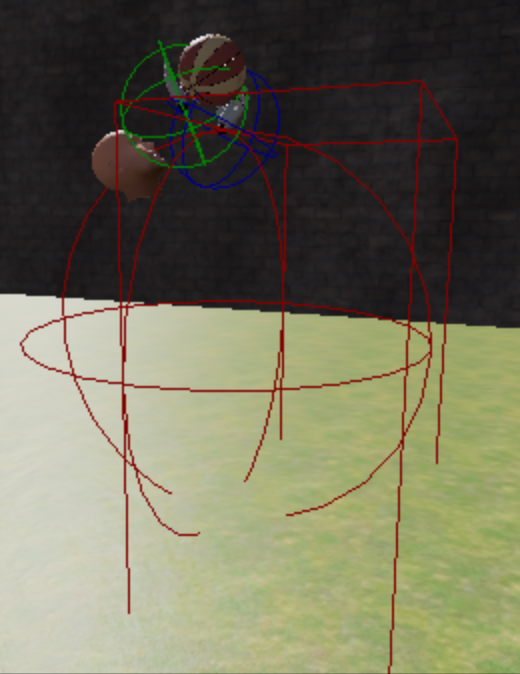
\includegraphics[width=1.0\linewidth]{PlaybackActor.png}
\caption{Beispiel einer Wiedergabe mit den drei Hüllkörpern. Die Kugeln um die Hände sind hier blau und grün dargestellt. Die Halbkugel für den Körper wird aus dem Schnitt des roten Quaders und der roten Kugel gebildet, da die Unreal Engine keine Halbkugeln als Hüllkörper anbietet.}
\label{fig:playback-actor}
\end{figure}
Bei der Wiedergabe werden das HMD und die Controller durch Modelle von Kopf und Händen dargestellt. Sie besitzen Hüllkörper mit denen die Gegenstände in der Nähe der Hände bzw. des Körpers ermittelt werden. Sie repräsentieren somit wie in \cite{scene-grok} die \textit{aktiven Objekte}. Wir verwenden hierzu ebenfalls Kugeln für die Hände und eine Halbkugel, die vom Kopf senkrecht nach unten verläuft für den Bereich vor dem Körper (Siehe Abbildung \ref{fig:playback-actor}. Hier ist die Tasse in der rechten Hand ein aktives Objekt). Die Radien sind über die Einstellungen anpassbar. Zudem können bei der Wiedergabe zugleich die Merkmalsvektoren mit berechnet werden.

\subsection{Mermalsvektoren erstellen}
Welche Merkmale verwendet werden sollen wird im Quelltext angegeben. Die Unreal Engine bietet mit den sogenannten Blueprints eine graphenbasierte Alternative zur C++-Programierung an. Die von uns erstellte Blueprintfunktion \glqq{}logFeatures\grqq{} hat als Inputparameter die Kalibrierungsdaten, alle Informationen zu Kopf und Händen und einen Liste mit den Featurevektoren, an den jeder neu berechnete Vektor angehangen wird. Ein kurzes Beispiel ist in Abbildung \ref{fig:log-features} zu sehen. Dort werden als Merkmale die Höhe des Kopfes und dessen Abstände zu den beiden Händen berechnet. Dafür wird zunächst die Raumposition (\glqq{}GetWorldLocation\grqq{}) der Händen und des Kopfs bzw. deren Hauptkomponenten (\glqq{}Default Scene Root\grqq{}) ausgelesen. Das erste Merkmal ist die Z-Komponente, also die Höhe des HMDs über dem Boden, dividiert durch die zuvor in der Kalibrierung gemessene Höhe des Nutzers. Die Merkmale zwei und drei ergeben sich aus dem euklidischen Abstand zwischen dem Kopf und den Händen. Auch hier wird zur Normierung durch die zuvor gemessene Armlänge geteilt. Die Merkmale werden zusammengefasst und an die Liste mit den vorherigen Merkmalsvektoren angehangen. Die von uns verwendeten Mermale werden im Abschnitt \ref{sec:features} genauer beschrieben.
\begin{figure}[hbtp]
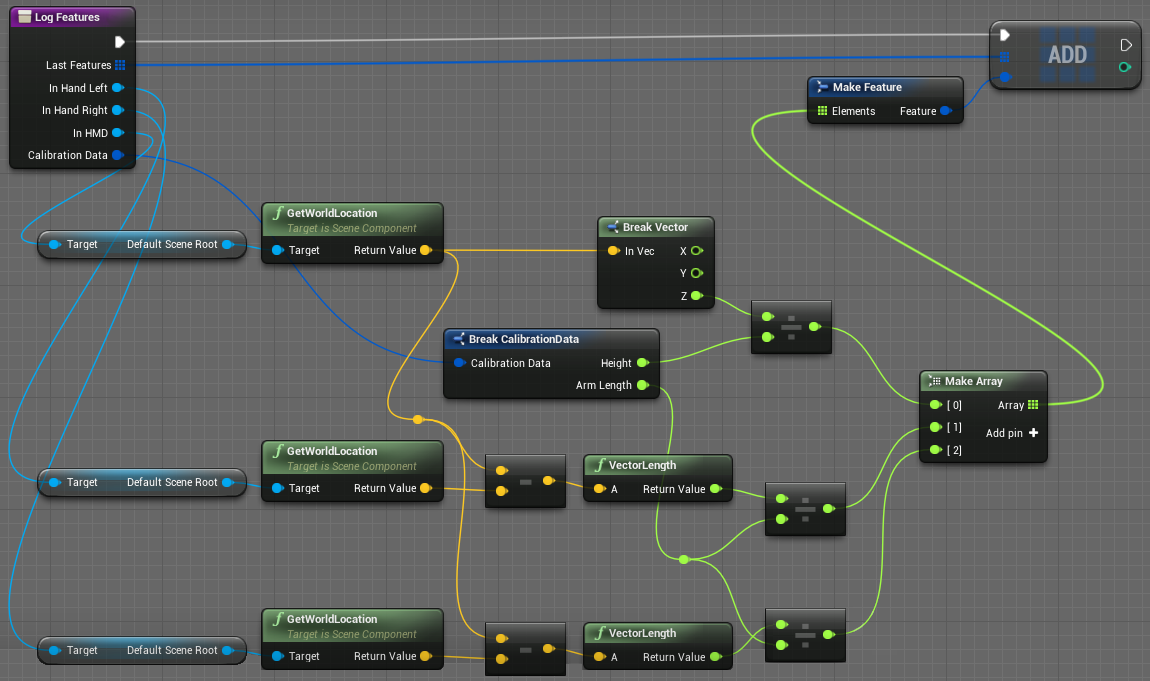
\includegraphics[width=1.0\linewidth]{LogFeatures.png}
\caption{Merkalsvektoren im Blueprint erstellen}
\label{fig:log-features}
\end{figure}

\subsection{Trainings- und Testdaten erstellen}
Nachdem die Featurevektoren herausgeschrieben wurden kann das Trainingsmodell erstellt werden. Hierfür verwenden wir die Support-Vector-Machine libsvm \cite{libsvm}. Um das Modell zu generieren benötigt die SVM Trainings- und Testdaten, die wir aus den aufgenommen Merkmalsvektoren erstellen. Diese liegen in dem Unterordner \glqq{}Features\grqq{} des Aufnahmeverzeichnisses. Zu jeder Aufnahme existiert eine entsprechende Datei mit den Featurevektoren. Da die libsvm nur Zahlen als Label der Aktionen verwendet, befindet sich dort zudem eine Datei die jeder Gruppe von Aktionen einen Index zuordnet. Mit einem Skript können die Hälfte der Aufnahmen jeder Gruppe in einer Testdatei und die andere Hälfte in einer Trainingsdatei zusammengefügt werden. Aus den Trainingsdaten erstellt die libsvm im Anschluss ein Trainingsmodell, auf dessen Grundlage die Klassifizierung der Test- bzw. Livedaten erfolgt.

\subsection{Live Klassifizierung}
Bei der Live Klassifizierung werden vom Benutzer Aktionen ausgeführt und daraus in Echtzeit die Featurevektoren bestimmt. Zu diesem Zweck haben wir die libsvm über C++ an das Framework angebunden ist. Zu Beginn wird das zuvor generierte Klassifizierungsmodell von der SVM geladen. Während der Live Klassifizierung werden dann, wie zuvor beim Erstellen der Trainingsdaten, in regelmäßigen Abständen die Merkamlsvektoren für den aktuellen Zeitpunkt berechnet. Die SVM wertet jeden Featurevektor auf der Grundlage des trainierten Modells aus und prognostiziert die Art der dargestellten Aktion. Wir stabilisiern das Ergebnis im Anschluss noch, indem immer die Prognose ausgeben, die unter den letzten 10 Klassifizierungen am häufigsten aufgetreten ist. 


\section{Support Vector Machine SVM}

\subsection{Einführung}
Eine Support Vector Machine führt eine Klassifikation von Objekten anhand von bereits Klassifizierten Objekten aus. Die Objekte werden als n-dimensionale Vektoren $v$ im Objektraum $X \subseteq \mathbb{R}^{n} $ dargestellt, bei denen je ein Wert ein bestimmtes Merkmal (hier Feature) des Objektes darstellt. Zur Klassifizierung wird der Objektraum durch Hyperebenen so geteilt, das jede Klasse von den anderen getrennt ist. Das heißt es erfolgt eine Zuordnung des Objektraumes $X$ zum Ergebnisraum $Y = {1,...,m} \subseteq \mathbb{R}$, der alle Klassen beinhaltet. Zur Berechnung dieser Hyperebenen dienen die Trainingsdaten $T =((x_{1},y_{1}),...,(x_{l},y_{l})) \subseteq (X \times Y)$, die der SVM übergeben werden. Somit besteht jedes Trainingsset aus einem Objekt $x_{i} \in X$ und der dazugehörigen Klasse $y_{i} \in Y$. Die Hyperebenen werden so gewählt, das der möglche Unterschied innerhalb einer Klasse möglichst groß ist. Dies wird dadurch realisiert, dass die Abstände der Vektoren, die der Hyperebene am nächsten liegen maximiert werden (Maximum Margin). Diese der Hyperebene am nächsten liegenden Vektoren werden Support-Vectors genannt, da durch diese die optimale Hyperebene ""stabilisiert" wird. Jedoch lassen sich nicht alle Datenpunkte durch Hyperebenen trennen, da es Ausreißer geben kann und Klassen sich teilweise sogar überschneiden. Um diese Daten zu klassifizieren, bedient sich die SVM des Kernel-Tricks.

\subsection{Lineare Klassifikation}
Die einfachste Art der Linearen Klassifikation ist die binäre Klassifikation. Hierbei werden die Vektoren mit Hilfe der Funktion $ f: X \subseteq \mathbb{R} \rightarrow \mathbb{R} $ der positiven $ (f(x)>0) $ oder negativen $ (f(x)<0) $ Klasse zugeordnet. Die trennende Hyperebene lässt sich durch einen Normalenvektor $\vec{\omega} \in X$ und ein Offset $b$ beschreiben.
Damit gilt:\[ f(\vec{x})=\left\langle \vec{\omega} \cdot \vec{x} \right\rangle\ + b = \sum\nolimits_{i=1}^n \omega x + b \]
Mit der Entscheidungsfunktion $h : \mathbb{R} \rightarrow \{-1,1\}$:
\[ h(x) = sign(f(x)) = sign (\sum\nolimits_{i=1}^n \omega x + b)\]
Eingabevektoren, die sich auf diese Weise trennen lassen werden linear separabel genannt.

\begin{figure}[hbtp]
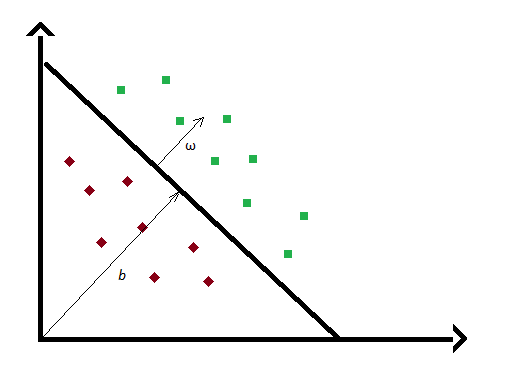
\includegraphics[width=0.7\linewidth]{LinSeparabel.png}
\centering
\caption{In Abbildung 3 ist ein Beispiel für Linear separierabare Eingabevektoren zu sehen. Diese werden mit Hilfe von h(x) in 2 Klassen überhalb (positiv bzw. grün) und unterhalb (negativ bzw. rot) der Geraden eingeteilt. $\omega$ bestimmt hierbei die Steigung der Geraden, während $b$ sie parallel verschiebt.}
\label{fig:LinSeparabel}
\end{figure}
%%%%%%%%%%%%%%%%%%%%%%%%%%%%%%%%%%%%%%%%%%%%%%%%%%%%%%%%%%%%

\section{Limitationen}
Wie im vorherigen Abschniit verwenden wir die Kopfhöhe und den mininmal und maximalen Abstand der Hand zum Kopf. Diese werden in unserem Fall 5 mal in der Sekunde aufgenommen und beschreiben so die dargestellte Pose. Eine Aktion ist eine geordnete Abfolge dieser Merkmale. Wir haben aber die Reihenfolge der Merkmalen beim Trainieren unser SVM nicht berücksichtigt. Die Merkmalsvektoren sind daher auch bei verschiedenen Aktionen oftmals recht ähnlich. In Abbildung \ref{fig:??} ist das gut zu erkennen. Hier liegen die Merkmale der Aktionen Basketball (?rot?) und Trinken (?blau?) nah zueinander, da sowohl beim Basketball als auch beim Trinken eine Nickbewegung des Kopfes ausgeführt wird.

\subsection{Gewicht als Schwerpunkt zur Klassifikation}
Auf Grund der Ähnlichkeit fällt in diesen Fällen die Masse des nächsten Gegenstandes stärker ins Gewicht. Haben dann die Szenenobjekte ähnliche Massen, wie die Getränkeflasche und der Basketball, kann das zu Fehlklassifizierungen führen.  Wird zum beispiel im Stehen aus der Flasche getrunken, so kann die Aktion fälschlicherweise als "Basketball spielen" klassifiziert werden. 



\section{Ausblick und Diskussion}
Wir haben eine Methode zur Erforschung der Aktionen vom Menschen in virtueller Realität vorgestellt. Diese Methode bildet Mermalsvektoren aus der Pose eines Menschs und den Eigenschaften der Gegenstände aus der Szene und verwendet dabei eine SVM als Klassifizierer. Um die Pose der durchführenden Person darzustellen, wurden die Kopfhöhe und die Abstände von den Händen zum Kopf genutzt und unter Berücksichtigung der Körpermaße des Nutzers kalibriert.

\subsection{Machinelles Lernen kombiniert mit Automaten}
Da wir die Reihenfolge der Merkmalvektoren in Relation mit den Aktionen nicht berücksichtigen, bietet es sich an die Pose in Zustände zu unterteilen und die Reihenfolge der verschiedenen Zuständen und die jeweilige Interaktion mit den Gegenstäden als eine Aktion zu betrachten. (nicht sicher ob wir so was machen möchten). Damit sollte die verwendete SVM in der Lage sein nicht lineare multidimensionale Funktionen von einander zu unterscheiden (wenn man noch live Klassifizieren möchte!)



%%%%%%%%%%%%%%%%%%%%%%%%%%%%%%%%%%%%%%%%%%%%%%%%%%%%%%%%%%%%

